\documentclass{article}

\usepackage[utf8]{inputenc} % allow utf-8 input
\usepackage[T1]{fontenc}    % use 8-bit T1 fonts
\usepackage{hyperref}       % hyperlinks
\usepackage{amsfonts}       % blackboard math symbols
\usepackage[margin=2cm]{geometry} % margins of document
\usepackage{multicol} % multi columnas
\usepackage{graphicx} % Images
\graphicspath{ {./images/} }


\title{CIRCULACIÓN CON DEMANDAS \\ Proyecto Final \\ \line(1,0){500}}
	\author{
	  \textbf{Alejandro Vargas Aldaco} \\ \\
	  Análisis de Algoritmos 2019-2 \\
	  Profesor: Carlos Zerón \\
	  Ayudante: Antonio Galván
	}
	\date{Junio 8, 2019 \\ \line(1,0){500}}
	

\begin{document}
\maketitle

\setlength{\parindent}{0cm} 
\setlength{\parskip}{.4cm}


\begin{section} {Fundamentos y consultas}
	
	\begin{subsection}{Describe con detalle en que consiste el Problema de Circulaciones con Demandas o una variante de él.}
		
		El problema de la circulación con demandas en sí, es una extensión generalizada del problema de máximo flujo. Si bien hay varios problemas en programación lineal o programación entera que no son instancias directas del problema de máximo flujo. Éstas se pueden modelar como una gráfica, en donde existen varias fuentes y varios sumideros.
		
		Por ejemplo, una cadena de agencias de autos necesita que le distribuyan a cada una de sus sucursales cierta cantidad de autos, con diferentes modelos, etc. Existen varias plantas distribuidoras de autos con las cuales se puede satisfacer la demanda de las sucursales de las agencias.
		
		En este caso el algoritmo del máximo flujo no es capaz de resolver el problema si se plantea de esta manera, ya que para que se pueda modelar el problema como una instancia del máximo flujo, es indispensable que sólo haya una fuente y un sumidero. En el problema de la circulación con demandas, y en este caso hay varias fuentes, que son las plantas distribuidoras, y varios sumideros, que son las agencias de los autos.  Para generalizar el problema de máximo flujo lo que se hace es crear una super fuente que es la que se encarga de darle flujo a todas las fuentes y un super sumidero que es la que recibe el flujo de todos los sumideros. 
		
		Es decir, a partir de la gráfica del problema original, se crea una nueva gráfica que contiene la misma estructura, pero se le añaden la superfuente y el supersumidero. Los números dentro de los nodos son la demanda y y los números en las aristas son las capacidades y valores del flujo. Al hacer estas modificaciones, el resultado es una instancia del problema del máximo flujo.
		
		El problema de la circulación con demandas se puede resumir a satisfacer toda la demanda. Pero en muchas aplicaciones, no sólo se requiere satisfacer demandas en varios nodos; También se necesita forzar el flujo para hacer uso de ciertas aristas. Esto se puede hacer colocando límites inferiores en las aristas, así como los límites superiores habituales impuestos por las capacidades de las aristas. Y esta generalización es llamada, en inglés, "Circulation with demandas an lower bounds".
		
	\end{subsection}
	
	\begin{subsection}{Proporciona una descripción sobre el diseño del algoritmo mencionado en la sección para resolver dicho problema.}
		
		La estrategia, que usa para resolver el problema de circulación con demandas, es reducir el problema a encontrar una circulación factible con demandas $\{dv\}$ al problema de encontrar un flujo máximo en una gráfica con una superfuente y un supersumidero. Es decir a partir de la gráfica $G$ del problema original, se crea otra $G'$ agregando la superfuente y el supersumidero y se resuelve $G'$ como un problema de máximo flujo. 
		
		Decimos que la circulación con demandas $\{dv\}$ es una función que asigna un número real no negativo a cada arista y satisface las siguientes dos condiciones.
		
		(i) (Condiciones de capacidad) Para cada $e\in E$ tenemos $0 \leq f(e) \leq ce$. El flujo de la arista es menor o igual a su capacidad.
		
		(ii) (Condiciones de demanda) Para cada $ v \in V $ tenemos v, $f_{in}(v) - f_{out}(v) = dv$. Lo que entra por el nodo menos lo que sale de él es igual a su demanda.
		
		Entonces para la creación de $G'$, (i) considera lo que se debe cumplir para el algoritmo del máximo flujo. (ii) determina la demanda, y en este caso tenemos tres variantes:
		
		1. $dv < 0; v$ es una fuente.
		
		2. $dv > 0; v$ es un sumidero.
		
		3. $dv = 0; v$ es un nodo regular.
		
		Entonces, se crea un nodo $s*$ que será la superfuente y para cada nodo $v \in G$ tal que $v$ sea fuente se crea una arista dirigida $e$ de $s* \rightarrow v$ de tal manera que $ce = |dv|$. Analogamente, para crear el supersumidero, se crea un nodo $t*$ y para cada nodo $v \in G$ tal que v sea sumidero se crea una arista dirigida $e$ de $v \rightarrow t*$ de tal manera que $ce = |dv|$. Y el grafo resultante es $G'$.
		
	\end{subsection}
	
	\begin{subsection}{Desglosa la demostración de integridad del algoritmo.}
		
		Si consideramos una instancia arbitraria del problema de circulación, aquí hay una condición simple que debe cumplir para que exista una circulación factible: la oferta total debe ser igual a la demanda total.
		
		Proposición: si existe una circulación con demandas factible $\{dv\}$, entonces $\sum_{v}dv = 0$.
		
		Demostración: Supongamos que existe una circulación factible. Entonces $\sum_{v} dv = \sum_{v} f_{in} (v) - f_{out} (v)$. El valor $f(e)$ para cada borde $e = (u, v)$ se cuenta exactamente dos veces: una vez en $f_{out}(u)$ y una vez en $f_{in}(v)$. Estos dos términos son iguales; y como esto se mantiene para todos los valores $f(e)$, la suma global es 0.
		
		Como consecuencia de lo anterior tenemos que $\sum_{v:dv > 0} dv = - \sum_{v:dv<0} dv$. Sea D el valor común.
		
		Veamos que no puede haber un flujo de $s* \rightarrow t*$ mayor que D. Veamos que $ds* = \sum_{s*} f_{in} (s*) - f_{out} (s*)$ como $f_{in} (s*) = 0 \Rightarrow f_{out} (s*) = -ds*$. Por otro lado $dt* = \sum_{t*} f_{in} (t*) - f_{out} (t*)$ como $f_{out} (t*) = 0 \Rightarrow - \sum_{t*} f_{in} = -dt*$. Por propiedades de conservación, para cada nodo diferente de $s*$ y $t*$ se tiene que $\sum_{e \ into \ v} f(e) = \sum_{e \ out \ v} f(e)$. Como $s*$ es la única superfuente y $t*$ es el único supersumidero y $dv = 0$ para $v \neq s*$ y $ v \neq t*$, entonces $f_{out} (s*) = \sum_{t*} f_{in} (t*) \Rightarrow ds* = -dt*$. Por lo tanto $\sum_{v:dv>0} dv = ds* = - dt* = - \sum_{v:dv<0} dv$. Como D es el valor común. Por lo tanto no puede haber un flujo mayor que D.
		
		A pesar de que el párrafo anterior pudo ser reemplazado con lo que dice el libro, quise hacer una parte de la demostración a mi modo, la ida y la vuelta por medio de la igualdad, espero que esté bien. En resumen se ha probado que:
		
		Existe una circulación factible con demandas {dv} en $G$ si y sólo si el máximo $s* \rightarrow t*$ fluje en $G'$ tiene un valor $D$. Si todas las capacidades y demandas en $G$ están integradas, y hay una circulación factible, entonces hay una circulación factible que tiene un valor entero.
		
		Por último la autora agrega sin demostrar: 
		
		Al final de la Sección 7.5, utilizamos el Teorema de corte mínimo de flujo máximo para obtener la caracterización (7.40) de gráficos bipartitos que no tienen coincidencias perfectas. Podemos dar una caracterización análoga para gráficos que no tengan una circulación viable. La caracterización utiliza la noción de corte, adaptada a la configuración actual. En el contexto de problemas de circulación con demandas, un $corte(A, B)$ es cualquier partición del conjunto de nodos $V$ en dos conjuntos, con la restricción de que en un lado de partición caen las fuentes y en otra los sumideros. Incluimos la caracterización aquí sin una prueba. (7.51) El gráfico $G$ tiene una circulación factible con demandas $\{dv\}$ si y sólo si para todos los $cortes(A, B)$, $\sum_{v \in B} dv \leq c(A,B)$
		
	\end{subsection}

	\line(1,0){500}

\end{section}

\begin{section}{Aplicación}
	
	Una cadena de tiendas que vende ciertos productos, hace sus pedidos directamente al fabricante según el reporte de cada tienda y los productos deben llegar directamente a las tiendas según lo indique el pedido. 
	
	Para el día X la tienda D requiere 10 productos y la tienda F requiere 11. El fabricante puede satisfacer el pedido de ambas tiendas de la siguiente manera:
	
	El almacen C le pueden enviar hasta 3 productos a la tienda D y a su vez le puede enviar hasta 10 productos al almacen A (No sé por qué pero así es su logística). Pero el día X sólo cuenta con 7 productos.
	
	El almacen A le puede enviar hasta 6 a la tienda D y hasta 7 al almacen E. Pero ese día sólo cuenta con 8.
	
	El almacen E le puede enviar hasta 4 al almacen B y hasta 4 a la tienda F. Pero ese día no cuenta con stock y solo dependerá de lo que le pueda enviar el almacen A.
	
	El almacen B le puede enviar hasta 7 a la tienda D y hasta 9 a la tienda F. Pero ese día sólo cuenta con 6 más lo que le pueda enviar el almacen 6.
	
	El problema a resolver es satisfacer la demanda de las dos tiendas con las limitantes con las que cuenta la logística implementada del fabricante.
	
	La gráfica del modelo del problema. Gráfica $G$ inicial.
	
	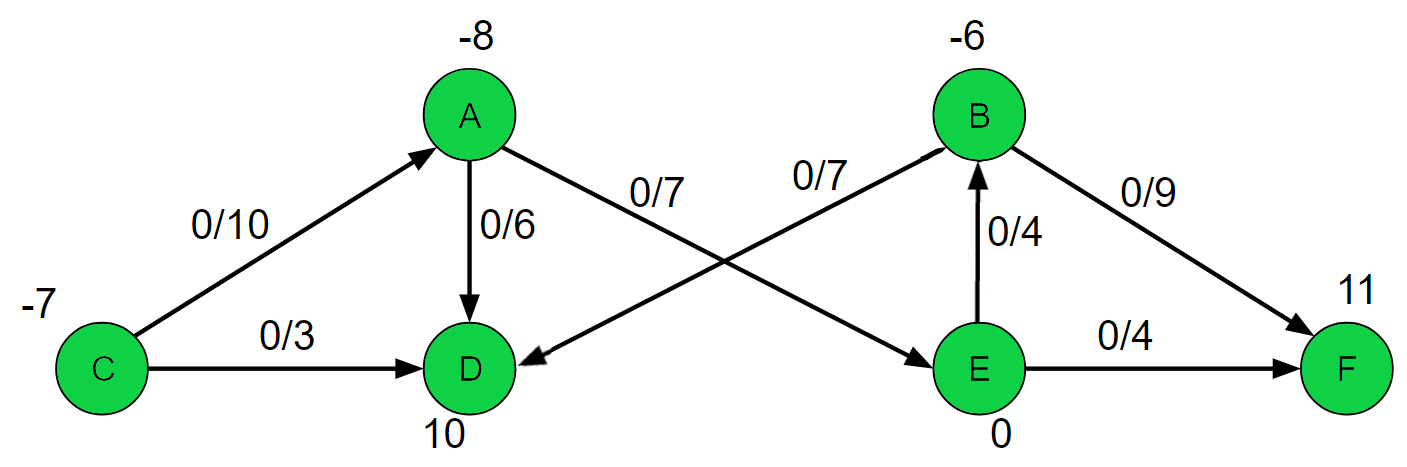
\includegraphics[width=\textwidth]{graph-initial}

	Una vez que se instancia la gráfica con los nuevos vértices $S$ y $T$, y se le aplica el algoritmo Ford Fulkerson, los resultados son los siguientes:
	
	\begin{multicols}{2}
		
		\centering Gráfica $G'$ con los vértices $S$ y $T$.
		
		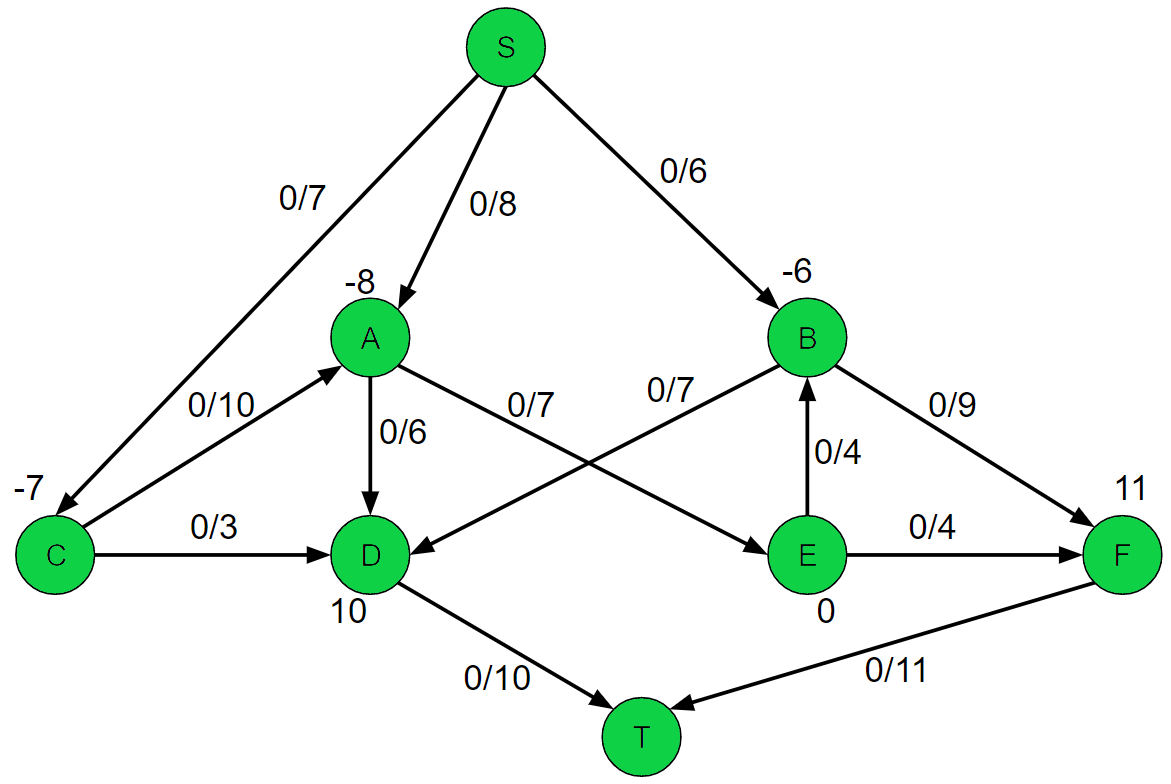
\includegraphics[width=0.48\textwidth]{graph-source-sink}
		
		Gráfica $G'$ con el máximo flujo.
		
		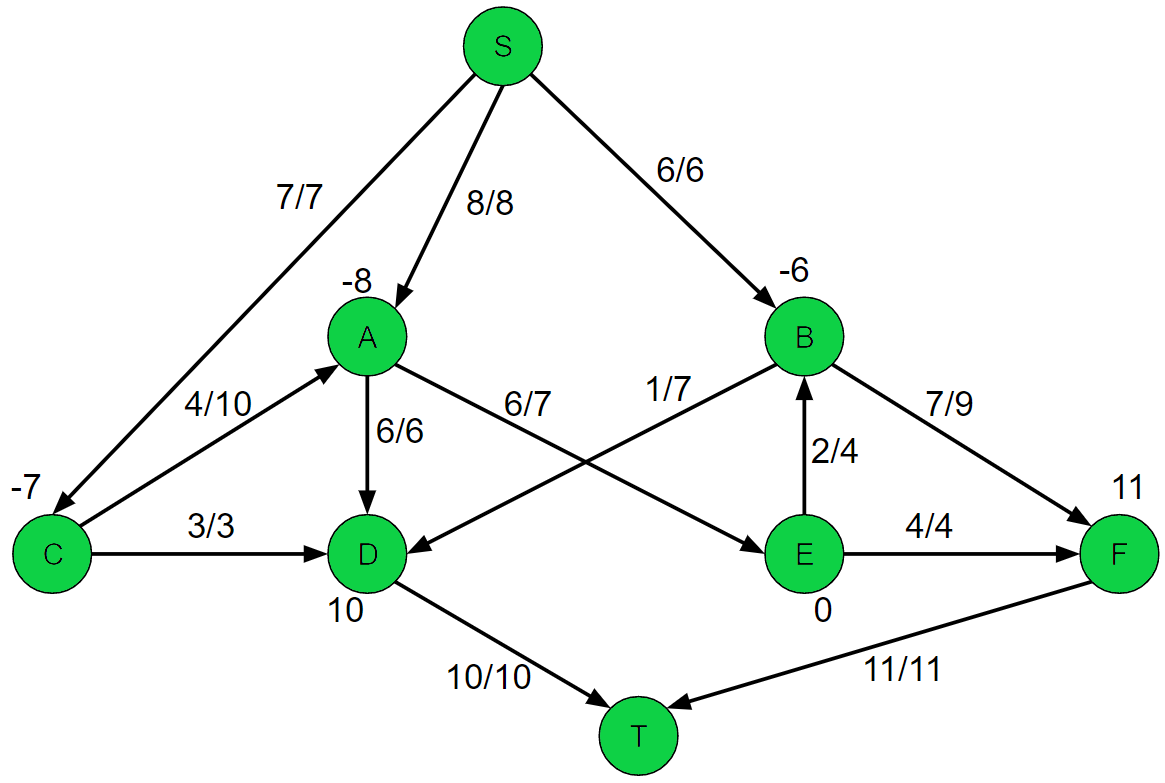
\includegraphics[width=0.48\textwidth]{graph-flows-assigned}
		
	\end{multicols}
	
	\line(1,0){500}
	
\end{section}

\begin{section} {Implementacón}
	
	La implementación es un proyecto Java, hecho con el ide Intellij, para almacenar los datos se requiere editar el archivo graph.txt que está en el root path del proyecto. Para editarlo se debe hacer de la siguiente manera:
	
	A cada nodo se le asigna un id:letra:demanda:arcos, nótese que el separador es el símbolo ":" (dos puntos). Para los arcos, cada arco se debe separa por el símbolo ";" (punto y coma). Cada arco se compone de dos números separados por "," (coma) idDestino,capacidad
	
	Por ejemplo la entrada por defecto es la del problema anterior
	
	0:A:-8:3,6;4,7\\
	1:B:-6:3,7;5,9\\
	2:C:-7:0,10;3,3\\
	3:D:10:\\
	4:E:0:1,4;5,4\\
	5:F:11:
	
	Para la primer línea:
	
	id : letra : demanda : idDestino , capacidad ; idDestino , capacidad\\
	0 : A : -8 : 3 , 6 ; 4 , 7
	
	Quiere decir que se trata del nodo A, con el id 0, tiene una demanda de -8 y tiene dos arcos 0 -> 3 (A -> D) con capacidad 6 y 0 -> 4 (A -> E) con capacidad 7.
	
	Si no tiene arcos se deja vacío como en 3 y 5;
	
	Cabe recordar que para que funcione el algoritmo, la oferta debe ser igual a la demanda. Los que utilizan otros métodos para resolver este tipo de problemas, lo que hacen es que si la demanda total es menor que la oferta total crean una demanda ficticia para compensar, algo así como lo que va a quedar en un stock simulado. En el caso contrario si la demanda total es mayor a la oferta total, lo que indica es que no hay suficiente stock para cubrir toda la demanda. El primer caso casi siempre se cumple.
	
	Ahora veamos el resumen de la salida del programa. Para ver los detalles de la gráfica residual, hay que ejecutar el programa, ya que la salida contiene más detalles.
	
	Ruta incrementable: S -> A -> D -> T, Capacidad mínima: 6.0
	
	Ruta incrementable: S -> B -> D -> T, Capacidad mínima: 4.0
	
	Ruta incrementable: S -> B -> F -> T, Capacidad mínima: 2.0
	
	Ruta incrementable: S -> A -> E -> F -> T, Capacidad mínima: 2.0
	
	Ruta incrementable: S -> C -> A -> E -> F -> T, Capacidad mínima: 2.0
	
	Ruta incrementable: S -> C -> D -> B -> F -> T, Capacidad mínima: 3.0
	
	Ruta incrementable: S -> C -> A -> E -> B -> F -> T, Capacidad mínima: 2.0
	
	Existe una circulación factible 
	
	Flujo máximo: 21.0
	
	Cortadura mínima: S
	
	Gráfica residual: ((6 -> 0, capacidad: 8.0, flujo: 8.0), (0 -> 3, capacidad: 6.0, flujo: 6.0), (0 -> 4, capacidad: 7.0, flujo: 6.0), (2 -> 0, capacidad: 10.0, flujo: 4.0), (6 -> 1, capacidad: 6.0, flujo: 6.0), (1 -> 3, capacidad: 7.0, flujo: 1.0), (1 -> 5, capacidad: 9.0, flujo: 7.0), (4 -> 1, capacidad: 4.0, flujo: 2.0), (6 -> 2, capacidad: 7.0, flujo: 7.0), (2 -> 0, capacidad: 10.0, flujo: 4.0), (2 -> 3, capacidad: 3.0, flujo: 3.0), (0 -> 3, capacidad: 6.0, flujo: 6.0), (1 -> 3, capacidad: 7.0, flujo: 1.0), (2 -> 3, capacidad: 3.0, flujo: 3.0), (3 -> 7, capacidad: 10.0, flujo: 10.0), (3 -> 7, capacidad: 10.0, flujo: 10.0), (0 -> 4, capacidad: 7.0, flujo: 6.0), (4 -> 1, capacidad: 4.0, flujo: 2.0), (4 -> 5, capacidad: 4.0, flujo: 4.0), (1 -> 5, capacidad: 9.0, flujo: 7.0), (4 -> 5, capacidad: 4.0, flujo: 4.0), (5 -> 7, capacidad: 11.0, flujo: 11.0), (5 -> 7, capacidad: 11.0, flujo: 11.0), (6 -> 0, capacidad: 8.0, flujo: 8.0), (6 -> 1, capacidad: 6.0, flujo: 6.0), (6 -> 2, capacidad: 7.0, flujo: 7.0), (3 -> 7, capacidad: 10.0, flujo: 10.0), (3 -> 7, capacidad: 10.0, flujo: 10.0), (5 -> 7, capacidad: 11.0, flujo: 11.0), (5 -> 7, capacidad: 11.0, flujo: 11.0))
	
	
\end{section}

\begin{section}{Referencias}
	\url{http://www.cs.sjtu.edu.cn/~jiangli/teaching/CS222/files/materials/Algorithm%20Design.pdf}
\end{section}

\end{document}